\documentclass[aspectratio=169,11pt]{beamer}

% Shared style (ib-tutorials.sty at the repo root).
\makeatletter\def\input@path{{./}{../}}\makeatother
\usepackage{ib-tutorials}

\usepackage[utf8]{inputenc}
\usepackage{amsmath,amssymb}
\usepackage{booktabs}
\usepackage{array}
\newcolumntype{L}[1]{>{\raggedright\arraybackslash}p{#1}}
\usepackage{graphicx}
\graphicspath{{../pictures/3-ibamr-fundamentals/}{pictures/3-ibamr-fundamentals/}}
\usepackage{xcolor}
\usepackage{listings}
\usepackage{tikz}
\usetikzlibrary{arrows.meta,positioning,shapes.geometric,fit,calc,decorations.pathmorphing}
\usepackage{hyperref}

\newcommand{\sourcecredit}[1]{\vfill\begin{flushright}\tiny\textcolor{DarkGray}{#1}\end{flushright}}

\lstset{
  basicstyle=\ttfamily\scriptsize\color{BlackGray},
  keywordstyle=\color{NavyBlue}\bfseries,
  commentstyle=\color{DarkGray}\itshape,
  stringstyle=\color{OliveGreen},
  showstringspaces=false,
  columns=fullflexible,
  keepspaces=true,
  breaklines=true,
  breakindent=1em,
  frame=single,
  framerule=0.4pt,
  rulecolor=\color{LightGray},
  backgroundcolor=\color{LightGray!30},
  xleftmargin=0.25em,
  xrightmargin=0.25em
}
\lstdefinestyle{shell}{morecomment=[l]{\#}}
\lstdefinestyle{input}{morecomment=[l]{//}}
\lstdefinestyle{matlab}{morecomment=[l]{\%}}
\lstdefinestyle{python}{morecomment=[l]{\#}}
\lstdefinestyle{data}{}
\lstdefinestyle{tiny}{basicstyle=\ttfamily\tiny\color{BlackGray}}
\lstdefinestyle{inputtiny}{morecomment=[l]{//},basicstyle=\ttfamily\tiny\color{BlackGray}}
\lstdefinestyle{matlabtiny}{morecomment=[l]{\%},basicstyle=\ttfamily\tiny\color{BlackGray}}
\lstdefinestyle{pythontiny}{morecomment=[l]{\#},basicstyle=\ttfamily\tiny\color{BlackGray}}
\lstdefinestyle{cpp}{language=C++,morecomment=[l]{//}}
\lstdefinestyle{cpptiny}{language=C++,morecomment=[l]{//},basicstyle=\ttfamily\tiny\color{BlackGray}}
\lstdefinestyle{cmake}{morecomment=[l]{\#}}

\title[Adding mass]{Adding mass}
\subtitle{The penalty immersed boundary method: points with mass, the \code{.mass} file, gravity, and a spider on its dragline}
\author[Miller]{Laura A. Miller}
\institute[UArizona]{Department of Mathematics, University of Arizona}
\date{Using IB Software \textbullet\ Part III \textbullet\ Chapter 13}

\begin{document}

% 1
\begin{frame}[plain]
\maketutorialtitlepanel{%
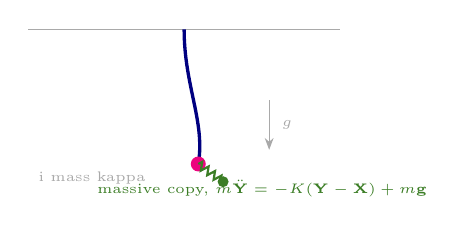
\begin{tikzpicture}[scale=0.9]
  \draw[DarkGray,thin] (0,2.4) -- (4.4,2.4);
  \draw[NavyBlue,very thick] (2.2,2.4) .. controls (2.2,1.6) and (2.5,1.1) .. (2.4,0.5);
  \fill[RubineRed] (2.4,0.5) circle (3pt);
  \draw[decorate,decoration={zigzag,segment length=1mm,amplitude=0.5mm},OliveGreen,thick] (2.4,0.5) -- (2.75,0.25);
  \fill[OliveGreen] (2.75,0.25) circle (2.2pt);
  \draw[-{Stealth[length=1.5mm]},DarkGray] (3.4,1.4) -- (3.4,0.7); \node[font=\tiny,text=DarkGray] at (3.65,1.05) {$g$};
  \node[font=\tiny,text=OliveGreen] at (3.3,0.15) {massive copy, $m\ddot{\mathbf{Y}} = -K(\mathbf{Y}-\mathbf{X}) + m\mathbf{g}$};
  \node[font=\tiny,text=DarkGray] at (0.9,0.3) {\code{i mass kappa}};
\end{tikzpicture}}
\end{frame}

% 2
\begin{frame}{Learning goals}
\label{fr:goals}
\footnotesize By the end of this chapter you should be able to:
\begin{enumerate}
  \item say why an ordinary IB point has no mass of its own (it moves with the fluid and the fluid carries the inertia) and what the penalty IB method adds: a massive copy of a point, tied to it by a stiff spring, that moves by Newton's law;
  \item write a \code{.mass} file (\code{index mass kappa}), choose the penalty stiffness, and switch a program from \code{IBMethod} to \code{PenaltyIBMethod} with gravity in the input block;
  \item run the spider-ballooning example (IB/12), a point mass on a massless dragline falling through air, and read the fall from the position files;
  \item know what the penalty stiffness does to the time step, what ``mass per unit depth'' means in 2D, and where IBAMR's other massive-body methods (constraint IB, IBFE with density) are the better tool.
\end{enumerate}
\begin{punchbox}
\footnotesize Everything in Part III so far was neutrally buoyant: the structure's mass was the fluid's. A falling spider, a sinking seed or a heavy wing needs mass of its own, and the penalty method is the way IBAMR's standard IB gives it.
\end{punchbox}
\end{frame}

% 3
\begin{frame}{How this chapter was checked}
\label{fr:checked}
\begin{itemize}\footnotesize
  \item The \code{.mass} file format, the \code{PenaltyIBMethod} input keys and the update of the massive copies are quoted from the IBAMR 0.19.0 sources (\code{IBStandardInitializer.h}, \code{PenaltyIBMethod.cpp}); the upstream example that uses the method (\code{examples/IB/explicit/ex3}) is named.
  \item The example IB/12 is the course's \code{8-AddingMass-Spider} (2020) ported to the CMake build and current IBAMR, with its generator's beam loop corrected and its unused temperature field removed; it builds with 0 warnings and runs, and the figure is from that run. The generator's Python and MATLAB versions write identical files (Octave 8.4 against Python 3.12).
  \item The 2020 lecture \emph{Adding mass to the boundaries} (IBAMR Lecture 8, the only deck on this topic) is quoted in full; its module name and folder typo are noted, not reproduced.
\end{itemize}
\begin{punchbox}
\footnotesize Slide numbers refer to this deck; chapter numbers (4e, 5, 6, 8a, 8b, 9b, 11, 15, 16, 19, 23) to the other chapters of this series.
\end{punchbox}
\end{frame}

% 4
\begin{frame}{Where to look things up}
\label{fr:lookup}
\small
\begin{itemize}
  \item \al{The method}: \code{include/ibamr/PenaltyIBMethod.h} and \code{src/IB/PenaltyIBMethod.cpp}; the massive copies' update is twenty lines (slide \ref{fr:update}).
  \item \al{The file format}: \code{include/ibamr/IBStandardInitializer.h}, the ``mass file format'' paragraph, quoted on slide \ref{fr:massfile}; the key \code{uniform\_bdry\_mass\_stiffness}.
  \item \al{The upstream example}: \code{examples/IB/explicit/ex3}, a filament with mass (chapter 9b used its force function; chapter 15 tours it).
  \item \al{The example of this series}: IB/12 spider ballooning (\code{main.cpp}, \code{generate\_mesh2d.py}/\code{.m}, \code{input2d}, README with the measured fall).
  \item \al{The physics}: Y. Kim and C. S. Peskin, \emph{Penalty immersed boundary method for an elastic boundary with mass}, Phys.\ Fluids 19 (2007) 053103; the lab's spider-ballooning papers (their research codes are not part of this repository).
  \item IB2d's massive points (chapter 4e) are the same idea in MATLAB and Python.
\end{itemize}
\end{frame}

% 5
\begin{frame}{Why an IB point has no mass, and how to give it some}
\label{fr:why}
\small
\begin{itemize}
  \item In the IB method (chapter 5) a point moves with the local fluid velocity, $\dot{\mathbf{X}} = \mathbf{U}(\mathbf{X})$, and spreads its force onto the fluid. The fluid's momentum equation carries all the inertia; the structure is a set of massless force-bearing points, neutrally buoyant by construction. That is right for a tissue in water and wrong for a spider in air.
  \item The \al{penalty IB method} (Kim and Peskin 2007) keeps the massless point $\mathbf{X}_i$ and adds a \al{massive copy} $\mathbf{Y}_i$ that does not interact with the fluid at all: it obeys Newton's law,
  \[
    m_i\,\ddot{\mathbf{Y}}_i = -K_i\,(\mathbf{Y}_i - \mathbf{X}_i) + m_i\,\mathbf{g},
  \]
  and a stiff spring of stiffness $K_i$ and zero rest length ties the two together. The massless point feels the equal and opposite force $+K_i(\mathbf{Y}_i - \mathbf{X}_i)$ and spreads it onto the fluid.
  \item If $K_i$ is large the copy follows the point closely, and the force transmitted is $m_i\ddot{\mathbf{Y}}_i - m_i\mathbf{g} \approx m_i\ddot{\mathbf{X}}_i - m_i\mathbf{g}$: the point behaves as if it had mass $m_i$ and weight $m_i\mathbf{g}$. The penalty is the price of not solving a coupled system: a stiff spring and a short time step.
\end{itemize}
\begin{punchbox}
\footnotesize Mass and gravity enter only through the copies. Points without a \code{.mass} line are the ordinary massless points; a structure can mix the two, as the spider does (a massless line, one massive point).
\end{punchbox}
\end{frame}

% 6
\begin{frame}{The 2020 lecture: the files, including \code{.mass}}
\label{fr:files}
\small From \emph{IBAMR Lecture 8: Adding mass to the boundaries} (2020), repeating the 2012 FAQ: ``In addition to the \code{input2d}/\code{input3d} files, there are a number of files that specify the initial conditions and material properties of the immersed elastic structures. The only such file that is required is the \code{.vertex} file, which specifies the initial positions of the IB points. There are several additional files that may be optionally specified:
\begin{itemize}
  \item A \code{.spring} file can be used to specify an essentially arbitrary network of linear or nonlinear springs that connect the various IB points. Each `spring' connects precisely two IB points.
  \item A \code{.beam} file can be used to specify a collection of linear beams with a preferred curvature. Each `beam' connects precisely three IB points.
  \item A \code{.target} file is used to specify IB points that are, by default, `tethered' by stiff linear springs to their initial positions.
  \item A \code{.mass} file is used to specify any additional mass associated with the IB points. For such files to have any effect, it is necessary that the IB solver be run in `penalty-IB' mode.''
\end{itemize}
\vspace{1mm}
\footnotesize The 2012 FAQ also listed a \code{.anchor} file (``anchor points neither apply force to the fluid nor interpolate velocity from the fluid; they are literally anchored in place''), which chapter 6 covers; the 2020 lecture left it out.
\end{frame}

% 7
\begin{frame}[fragile]{The \code{.mass} file format}
\label{fr:massfile}
\begin{columns}[T,onlytextwidth]
\begin{column}{0.5\textwidth}
\footnotesize ``Mass point input files end with the extension \code{.mass} and have the following format:
\begin{lstlisting}[style=data]
M                        # number of mass points in the file
i_0   mass_0   kappa_0   # vertex index, point mass, penalty spring constant
i_1   mass_1   kappa_1
i_2   mass_2   kappa_2
...
\end{lstlisting}
Note: mass points are anchored to `ghost' massive particles by linear springs with the specified spring constants and with zero resting lengths. The massive particles are `isolated' and simply move according to Newton's laws. The penalty parameter provides control over the energetic penalty imposed when the position of the Lagrangian immersed boundary point deviates from that of its massive copy.'' (2020, and \code{IBStandardInitializer.h} in 0.19.0, word for word)
\end{column}
\begin{column}{0.48\textwidth}
\begin{lstlisting}[style=data]
1
170 2.0000000000000000e-05 2.0000000000000000e+01
\end{lstlisting}
\footnotesize IB/12's \code{spider2d\_256.mass}: one massive point, the last point of the dragline (index 170 of 171), mass $2\times10^{-5}$ kg per unit depth, penalty stiffness $20$ N/m.
\begin{itemize}
  \item the index is the point's number within the structure's own files, as in every other file of chapter 6; the initializer checks it is in range;
  \item \code{uniform\_bdry\_mass\_stiffness} in the structure's input block overrides every line's \code{kappa}, like the other \code{uniform\_*} keys; there is no uniform mass;
  \item the file is read by \code{IBStandardInitializer} like the others, but its data are used only by \code{PenaltyIBMethod}: with the plain \code{IBMethod} the file is read and the masses do nothing (``for such files to have any effect\ldots'').
\end{itemize}
\end{column}
\end{columns}
\end{frame}

% 8
\begin{frame}[fragile]{Switching the program to the penalty method}
\label{fr:program}
\begin{columns}[T,onlytextwidth]
\begin{column}{0.52\textwidth}
\small ``\code{Main.C}'' (2020): the headers, with the one that matters last:
\begin{lstlisting}[style=cpptiny]
#include <ibamr/IBExplicitHierarchyIntegrator.h>
#include <ibamr/IBMethod.h>
#include <ibamr/IBStandardForceGen.h>
#include <ibamr/IBStandardInitializer.h>
#include <ibamr/INSCollocatedHierarchyIntegrator.h>
#include <ibamr/INSStaggeredHierarchyIntegrator.h>
#include <ibtk/AppInitializer.h>
#include <ibtk/LData.h>
#include <ibtk/LDataManager.h>
#include <ibtk/muParserCartGridFunction.h>
#include <ibtk/muParserRobinBcCoefs.h>
#include <ibamr/PenaltyIBMethod.h>
\end{lstlisting}
\small and the construction:
\begin{lstlisting}[style=cpptiny]
Pointer<PenaltyIBMethod> ib_method_ops = new PenaltyIBMethod("PenaltyIBMethod",
    app_initializer->getComponentDatabase("PenaltyIBMethod"));
\end{lstlisting}
\end{column}
\begin{column}{0.46\textwidth}
\scriptsize That is the whole change to the program: \code{PenaltyIBMethod} is derived from \code{IBMethod}, so the rest of \code{main.cpp} (the integrator, the initializer, the force generator, the output) is IB/01's unchanged. IB/12's \code{main.cpp} differs from IB/01's in the include and these two lines.
\vspace{1mm}

\footnotesize And in the input file (2020):
\begin{lstlisting}[style=inputtiny]
IBStandardInitializer {
   max_levels = MAX_LEVELS
   structure_names = "spider2d_256"
   spider2d_256 {
      level_number = MAX_LEVELS - 1
   }
}

PenaltyIBMethod {
   delta_fcn      = DELTA_FUNCTION
   enable_logging = ENABLE_LOGGING
   gravitational_acceleration = 0.0,-9.8
}
\end{lstlisting}
\scriptsize The block is named after the class (chapter 7's rule); \code{gravitational\_acceleration} is a vector with \code{NDIM} entries, in m/s$^2$, and applies to the massive copies only. Without the key, $\mathbf{g} = 0$ and the mass only adds inertia.
\end{column}
\end{columns}
\end{frame}

% 9
\begin{frame}[fragile]{What the method does each step, from the source}
\label{fr:update}
\begin{columns}[T,onlytextwidth]
\begin{column}{0.56\textwidth}
\begin{lstlisting}[style=cpptiny]
// src/IB/PenaltyIBMethod.cpp (0.19.0), the massive copies' half step (one of three places)
const double* const K = d_K_data[ln]->getLocalFormArray()->data();   // kappa of each mass point
const double* const M = d_M_data[ln]->getLocalFormArray()->data();   // its mass
...
for each mass point i, each direction d:
    Y_half = Y[NDIM * i + d] + 0.5 * dt * V[NDIM * i + d];           // the copy's position, a half step on
    X_half = ...                                                       // the IB point's position, a half step on
    V_new[NDIM * i + d] = V[NDIM * i + d]
        + dt * (-K[i] * (Y_half - X_half) / M[i] + d_gravitational_acceleration[d]);   // Newton's law
    Y_new = Y + dt * V_new ...
// and the penalty force on the IB point, added to the Lagrangian force before spreading:
F[NDIM * i + d] += K[i] * (Y[NDIM * i + d] - X[NDIM * i + d]);
\end{lstlisting}
\footnotesize (Condensed: the file has the loop three times, for the predictor, the midpoint and the corrector of the explicit integrator.) \code{K}, \code{M}, \code{Y} and \code{V} are Lagrangian data like \code{X} and \code{F}, created from the \code{.mass} file at start-up (\code{createLData("M")}, \code{createLData("K")}, \code{createLData("V")}).
\end{column}
\begin{column}{0.42\textwidth}
\scriptsize What to take from it:
\begin{itemize}
  \item the copy's velocity $\mathbf{V}_i$ is its own; the IB point's velocity is still interpolated from the fluid. At $t = 0$ the copy starts at $\mathbf{Y}_i = \mathbf{X}_i$ with the fluid's velocity;
  \item $K_i/m_i$ is the square of the spring--mass frequency $\omega_i$: the explicit update is stable only if $\Delta t\,\omega_i$ is small, $\Delta t < 2/\omega_i = 2\sqrt{m_i/K_i}$. The spider: $\sqrt{2\times10^{-5}/20} = 10^{-3}$ s, so $\Delta t = 5\times10^{-5}$ is twenty times below the limit;
  \item a stiffer $K_i$ keeps $\mathbf{Y}_i$ closer to $\mathbf{X}_i$ (the deviation at steady fall is $m_i g/K_i$: $10^{-5}$ m for the spider) at the price of a shorter step;
  \item the penalty force appears in the \code{F} files of chapter 11 like any other force on that point: its sum over a falling structure balances the fluid's drag on it: the weight once the fall is steady, less while the mass still accelerates.
\end{itemize}
\end{column}
\end{columns}
\end{frame}

% 10
\begin{frame}{The 2020 example: a point mass attached to a string}
\label{fr:spider2020}
\small ``\al{Point mass attached to a string.} Look at example \code{8-AddingMass-Spider} in the examples folder. In this example, a mass is attached to the bottom of a string. The string resists bending (a little) and stretching and is massless. This is a simplified model of spider ballooning. The spider is represented as the point mass. The silk drag line is the string (massless). The spider falls to the bottom of the domain due to gravity. The dragline slows it down.'' (2020)
\vspace{1mm}

\small ``\al{Spider ballooning example.} Dragline: massless, resists stretching and bending. Body: zero body diameter (body drag neglected), prescribed mass. Flow profile: quiescent fluid; uniform flow at angle $\theta$ to the horizontal; lid-driven flow. $m$: mass, $D$: body diameter, $L$: thread length, $d$: silk diameter, $V$: background flow velocity, $\theta$: flow angle. In all simulations, the model is constructed as a point mass at the end of a massless, elastic silk drag line. We performed three types of simulations: free fall (settling), uniform background flow, and shear flow.'' (2020, with its vorticity figure ``for variations in Re'')
\vspace{1mm}

\footnotesize The lecture's example used ``the module \code{ibamr/2018-03}'' on the UNC cluster, and its folder was misspelt in the course files; IB/12 is the same model under the CMake build of chapter 3. The research versions (the lab's spider-ballooning papers; their codes are not part of this repository) add the flow profiles and a body of finite size.
\end{frame}

% 11
\begin{frame}[fragile]{The 2020 generator and input}
\label{fr:gen2020}
\begin{columns}[T,onlytextwidth]
\begin{column}{0.5\textwidth}
\small ``\code{generate\_mesh2d.m}: this matlab file creates the string made of vertices (\code{.vertex} file), the springs that connect pairs of vertices (\code{.spring} file), the beams that connect triads of vertices (\code{.beam} file), the mass at the end of the string. Note that this is a 2d simulation. The mass is actually a mass per unit length.'' (2020)
\begin{lstlisting}[style=matlabtiny]
L = 0.3;                      % length of computational domain (m)
N = 256;                      % finest grid cells across
drag_length = 0.10;           % drag line length (m)
npts_drag = ceil(2*(drag_length/L)*N);
kappa_spring = 2.0e1;         % spring constant (Newton)
kappa_beam = 5.0e-15;         % beam stiffness constant (Newton m)
mass = 0.00002;               % mass of the spider (kg), I had to estimate what a 2D "spider sheet" would weigh
...
target_fid = fopen([mesh_name num2str(N) '.mass'], 'w');
fprintf(target_fid, '%d\n', 1);
fprintf(target_fid, '%d %1.16e %1.16e\n', npts-1, mass, kappa_target*ds/(ds));
\end{lstlisting}
\end{column}
\begin{column}{0.48\textwidth}
\small ``\code{Input2d}'' (2020):
\begin{lstlisting}[style=inputtiny]
// physical parameters
W     = 0.3            // Domain width, meters
H     = 0.6            // Domain height, meters
MU    = 0.00001846     // air viscosity
RHO   = 1.177          // air density, kg/m^3

// grid spacing parameters
MAX_LEVELS = 3         // maximum no. levels in locally refined grid
REF_RATIO  = 4         // refinement ratio between levels
N = 16
\end{lstlisting}
\footnotesize The course's shipped input file differed from the slide (2 levels of ratio 2 on a coarse $128\times256$ grid, the same $256$ cells across the width), was periodic across the width with walls above and below, and ran 20 s at $\Delta t = 5\times10^{-5}$: 400,000 steps. It also carried a temperature field with a Boussinesq body force that the lecture never mentioned; IB/12 leaves it out (chapter 19 has thermal forcing where it belongs).
\end{column}
\end{columns}
\end{frame}

% 12
\begin{frame}[fragile]{IB/12, spider ballooning: what it is}
\label{fr:ib12}
\begin{columns}[T,onlytextwidth]
\begin{column}{0.52\textwidth}
\scriptsize A box $0.3$ m wide and $0.6$ m high of air ($\rho = 1.177$, $\mu = 1.846\times10^{-5}$), periodic across, no-slip top and bottom; $256\times512$ cells at the finest level ($\Delta x = 1.17$ mm, 2 levels of ratio 2). A vertical dragline of 171 points, $0.1$ m long, from $y = 0.5$ down to $0.4$ in the middle of the width: springs $K = 20$ N, beams $k_b = 5\times10^{-15}$ N m$^2$ (``a little''), no target points. Its last point carries the spider: mass $2\times10^{-5}$ kg per unit depth, penalty stiffness $20$ N/m, gravity $-9.8$ m/s$^2$.
\begin{lstlisting}[style=pythontiny]
# generate_mesh2d.py (IB/12): the mass file
with open(f"{mesh_name}{N}.mass", "w", newline="\n") as f:
    f.write("%d\n" % 1)
    f.write("%d %1.16e %1.16e\n" % (npts - 1, mass, kappa_mass * ds / ds))
\end{lstlisting}
\footnotesize $\Delta t = 5\times10^{-5}$ s, 2 s (40,000 steps), 40 frames; about 20 minutes on 3 cores.
\end{column}
\begin{column}{0.46\textwidth}
\scriptsize What happens: the spider's weight, $m g = 2\times10^{-4}$ N per unit depth, pulls its copy down; the copy drags the IB point, the point drags the dragline and the air. The line straightens behind the falling spider and its drag (and the spider's own, through the delta function's footprint, since the point has no body) sets a terminal speed; the 2020 model is a settling experiment.
\vspace{1mm}

\footnotesize Changes from the course version: CMake build, \code{IBTKInit}, the temperature field removed, \code{output\_data} added; the generator's beam loop fixed (it wrote one beam past the end of the line under a header that did not count it) and the mass point put on the last point (the course file said the one before); 2 s instead of 20; \code{DT} as a plain number.
\vspace{1mm}

\footnotesize The ``mass per unit length'' of the lecture is the ``per unit depth'' of chapter 8b: a 2D spider is a rod of spiders along the third axis, and $2\times10^{-5}$ kg/m is the lecture's estimate of what that weighs.
\end{column}
\end{columns}
\end{frame}

% 13
\begin{frame}{IB/12: the fall}
\label{fr:fall}
\begin{columns}[T,onlytextwidth]
\begin{column}{0.6\textwidth}
\centering
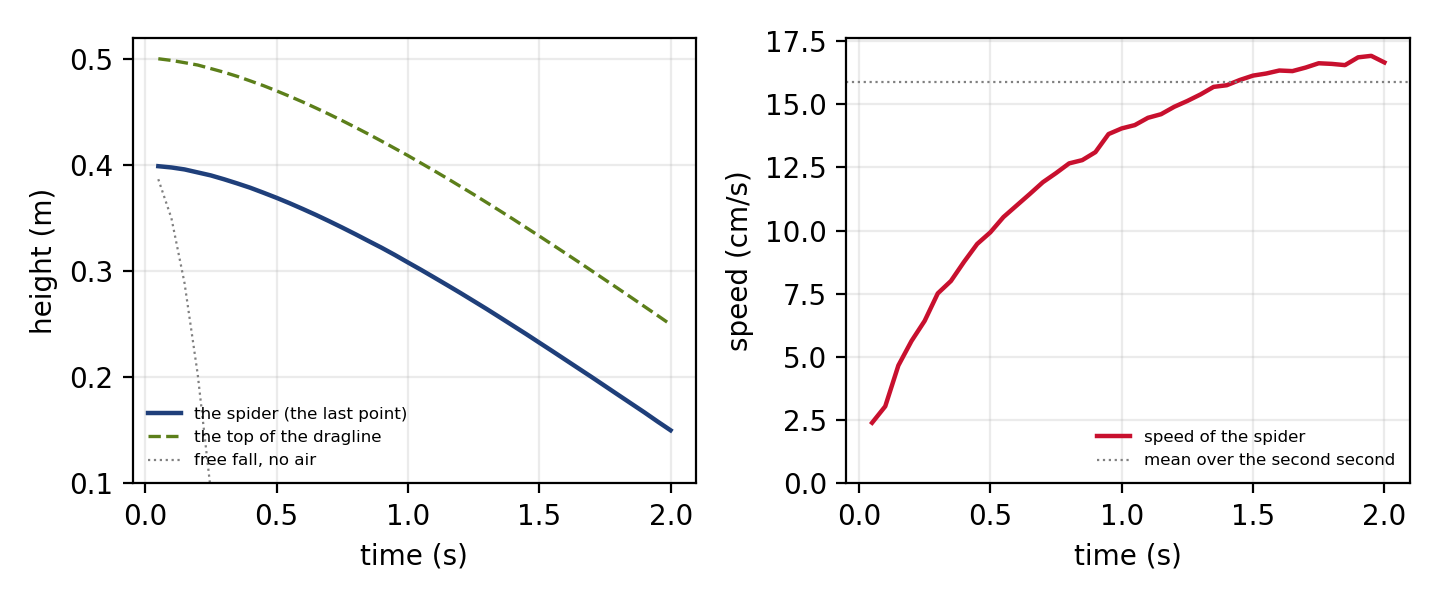
\includegraphics[width=\textwidth]{ch13-spider-fall}
\end{column}
\begin{column}{0.38\textwidth}
\scriptsize Left: the heights of the spider and of the top of the dragline against time, from the \code{X} files (chapter 11; the spider is the last point), with free fall for comparison. Right: the spider's speed from differences of positions.
\vspace{1mm}

\scriptsize Measured: the spider falls $1.0$ cm in the first quarter second, $9.2$ cm by $1$ s and $25.0$ cm by $2$ s; its speed rises from $3$ cm/s at $0.1$ s to $14$ cm/s at $1$ s and levels off near $17$ cm/s (mean $15.9$ cm/s over the second second), the terminal speed at which the air's drag on the line balances the weight. The top of the dragline falls by the same $25.0$ cm: the line keeps its length ($K = 20$ N stretches it by $10^{-5}$ m) and trails straight above the spider.
\end{column}
\end{columns}
\vspace{1mm}
\scriptsize The weight, $m g = 1.96\times10^{-4}$ N per unit depth, is what the \code{integral\{F\}} lines swing about from $t = 0.3$ s on ($-1.83$ to $-2.07\times10^{-4}$ N); the first, at $t = 0.05$ s, shows $-1.20\times10^{-4}$ N, while the spider still speeds up. The line's own springs cancel and only the penalty force is left (chapter 11): the massive copy's pull on the spider, $m(g - a)$.
\sourcecredit{IB/12 with IBAMR 0.19.0; \code{tools/ch13\_figures.py} reads \code{hier\_data\_IB2d/X.*}.}
\end{frame}

% 14
\begin{frame}{Choosing the mass and the penalty stiffness}
\label{fr:choosing}
\small
\begin{itemize}
  \item \al{Mass.} In 2D, per unit depth: the body's mass divided by its extent along the third axis, or (the lecture's way) an estimate of what a sheet of the body would weigh. Chapter 8b: what matters is the ratio of the body's mass to the fluid it displaces, $m/(\rho A)$ with $A$ its area, and the Froude or settling-speed scaling; a 2D model cannot get both the mass ratio and the drag right at once, so choose the one the question needs.
  \item \al{Added mass.} The fluid the body drags along is in the fluid equations already; do not add it to $m$.
  \item \al{Penalty stiffness.} Large enough that $\mathbf{Y} - \mathbf{X}$ stays small compared with the structure's size ($m g/K$ at steady fall, $m a/K$ in general), small enough for the step: $\Delta t < 2\sqrt{m/K}$, and in practice a tenth of that. With $K = 20$ and $m = 2\times10^{-5}$ the spider's copy lags by $10^{-5}$ m and the limit is $2\times10^{-3}$ s.
  \item \al{Several massive points.} A heavy wing or a sinking seed is a line or sheet of massive points: one \code{.mass} line per point, the mass divided among them, the same $K$ for all (\code{uniform\_bdry\_mass\_stiffness}).
  \item \al{Gravity on the fluid?} The key acts on the copies only. A density difference in the fluid itself (a plume) is a body force on the fluid (chapter 7, chapter 19), which is what the course code's Boussinesq term was.
\end{itemize}
\end{frame}

% 15
\begin{frame}{Other ways to give a body mass in IBAMR}
\label{fr:other}
\small
\begin{itemize}
  \item \al{Constraint IB} (\code{ConstraintIBMethod}, chapter 14): rigid bodies with mass and prescribed or free motion, solved as a constraint rather than a penalty; the right tool for a rigid sinking particle or a swimming rigid shape.
  \item \al{IBFE with a density difference} (Part IV, chapter 19): a finite-element body whose density differs from the fluid's carries its own inertia and weight through the momentum equation of the solid; no copies, no penalty, and the time step is the solver's.
  \item \al{Buoyancy as a force}: for a body that is nearly neutrally buoyant, a uniform body force on the structure ($\mathbf{F} = (\rho_s - \rho)\,V\,\mathbf{g}$ spread over its points, chapter 9b's \code{setUniformBodyForce}) gives the weight without the inertia, which is often all that matters at low Reynolds number.
  \item \al{IB2d} (chapter 4e) has massive points of the same penalty form, in MATLAB and Python, with gravity.
\end{itemize}
\vspace{1mm}
\begin{punchbox}
\footnotesize The penalty method is the simplest: one file, one class name, one key. It is also the one whose cost is a shorter time step for a stiff penalty, and whose inertia is only as good as the spring is stiff. Chapter 16 has the abort it produces when $\Delta t$ is too long.
\end{punchbox}
\end{frame}

% 16
\begin{frame}{What can go wrong}
\label{fr:wrong}
\scriptsize
\begin{tabular}{@{}L{0.3\textwidth}L{0.62\textwidth}@{}}
\toprule
The mistake & What happens\\
\midrule
\code{.mass} file with \code{IBMethod} & read and ignored: no weight, no inertia, no message (``for such files to have any effect\ldots'')\\
no \code{gravitational\_acceleration} key & $\mathbf{g} = 0$: the body has inertia but does not fall\\
\code{gravitational\_acceleration = -9.8} (one number) & a parse error: the key wants \code{NDIM} numbers\\
a penalty stiffness too large for $\Delta t$ & the copy and the point oscillate against each other and the run aborts within a few steps; $\Delta t < 2\sqrt{m/K}$\\
a penalty stiffness too small & the copy falls away from the point: the mass is where the point is not\\
the mass in kg for a 2D run & a body thousands of times too heavy per unit depth; divide by the depth, or estimate the sheet\\
added mass counted twice & a body that falls too slowly; the fluid is already there\\
a massive point index out of range & the initializer stops: ``vertex index \ldots is out of range''\\
a beam loop one triple too long (the course generator) & a beam naming a point that does not exist; the header count hides it until the file is checked\\
\bottomrule
\end{tabular}
\end{frame}

% 17
\begin{frame}{Homework}
\label{fr:hw}
\begin{columns}[T,onlytextwidth]
\begin{column}{0.56\textwidth}
\scriptsize From the 2020 course and this chapter (Appendix C collects the full set):
\begin{enumerate}
  \item IB/12: double the spider's mass and halve it; plot the three falls on one axes (chapter 11) and compare the terminal speeds with $m g$ against the drag.
  \item IB/12: lengthen the dragline to $0.2$ m (the generator's \code{drag\_length}) and shorten it to $0.05$ m; which falls slower?
  \item IB/12: raise the penalty stiffness to $200$ and lower it to $2$; measure $|\mathbf{Y} - \mathbf{X}|$ from the force on the mass point (the penalty force is $K(\mathbf{Y} - \mathbf{X})$), and find the step at which $200$ aborts.
  \item Put the spider in a uniform cross-wind (chapter 7's boundary conditions, a ramped \code{V}) as the 2020 study's second case, and in a shear flow as its third.
  \item Give IB/01's rubber band mass at every point (a \code{.mass} line each, the total mass of a $1$ mm-thick rubber ring per unit depth) and gravity; does it sink, and does it keep its shape?
\end{enumerate}
\end{column}
\begin{column}{0.43\textwidth}
\begin{punchbox}
\scriptsize What to hand in: the \code{.mass} lines, the input block, the step you used and the stability estimate, the height-against-time plot, and one VisIt frame with vorticity.
\end{punchbox}
\scriptsize Extension: compare IB/12 with a constraint-IB rigid body of the same mass (chapter 14).
\end{column}
\end{columns}
\end{frame}

% 18
\begin{frame}{Rules of thumb}
\label{fr:thumb}
\small
\begin{itemize}
  \item IB points are massless; mass lives on a copy tied by a penalty spring, and so does gravity.
  \item One line per massive point: \code{index mass kappa}; \code{PenaltyIBMethod} in the program and in the input, with \code{gravitational\_acceleration} as \code{NDIM} numbers.
  \item Mass per unit depth in 2D; no added mass.
  \item $\Delta t < 2\sqrt{m/K}$, use a tenth; $K$ large enough that $m g/K$ is small.
  \item The penalty force is in the \code{F} files; the sum over a falling body balances the fluid's drag on it: the weight once the fall is steady, less while the mass still accelerates.
  \item Rigid bodies: constraint IB. Dense elastic bodies: IBFE. Nearly buoyant: a body force.
  \item Check the generator's counts and indices before the first run.
\end{itemize}
\end{frame}

% 19
\begin{frame}{Summary}
\label{fr:summary}
\footnotesize
\begin{enumerate}
  \item The IB method's points are massless because the fluid carries the inertia; the penalty IB method adds a massive copy of a point that obeys Newton's law under gravity and is tied to the point by a stiff spring, so the point behaves as if it had the mass and the weight.
  \item The \code{.mass} file lists the points that get a copy, with their mass and penalty stiffness; \code{PenaltyIBMethod} replaces \code{IBMethod} in two lines of the program and one block of the input, where \code{gravitational\_acceleration} is set.
  \item The penalty stiffness trades closeness of the copy for the time step: $\Delta t < 2\sqrt{m/K}$.
  \item IB/12 is the 2020 spider: a point mass on a massless dragline settling through air; the fall is measured from the position files, and the example's corrections are listed.
  \item Constraint IB, IBFE with density, and a plain body force are the alternatives, each for a different question.
\end{enumerate}
\begin{homebox}
\footnotesize This ends the first part of Part III. Chapters 14 (constraint IB), 15 (the upstream examples) and 16 (what can go wrong, convergence tests and debugging) complete it.
\end{homebox}
\end{frame}

% 20
\begin{frame}{What changed since the older course notes}
\label{fr:changed}
\footnotesize
\begin{itemize}
  \item The lecture is quoted in full and the method behind it is explained from the source: the copies, Newton's law with gravity, the penalty force, the data arrays, and the stability limit, none of which the 2020 deck stated.
  \item The example is ported from a Makefile and a 2018 cluster module to the CMake build of chapter 3 and current IBAMR, its unused temperature field removed, its generator's beam loop and mass index corrected, output added, and the run shortened from 20 s to 2 s with the fall measured.
  \item ``Mass per unit length'' is tied to chapter 8b's per-unit-depth bookkeeping; the choice of mass and penalty stiffness has a slide; the alternatives (constraint IB, IBFE, a body force) are named.
  \item The folder typo and the retired module name are mentioned, not carried.
\end{itemize}
\end{frame}

% 21
\begin{frame}{Recordings (listed, not incorporated)}
\label{fr:videos}
\small The front matter's video list (chapter 0.1) has no recording of the 2020 \emph{Adding mass} lecture; it was the last of the 2020 IBAMR lectures and was taught from the slides quoted here.
\end{frame}

% 22
\begin{frame}{References}
\label{fr:refs}
\scriptsize
\begin{itemize}
  \item IBAMR 0.19.0: \code{include/ibamr/PenaltyIBMethod.h}, \code{src/IB/PenaltyIBMethod.cpp} (the copies' update, gravity), \code{include/ibamr/IBStandardInitializer.h} (the mass file format), \code{examples/IB/explicit/ex3} (a filament with mass). \url{https://github.com/IBAMR/IBAMR}
  \item Y. Kim and C. S. Peskin, \emph{Penalty immersed boundary method for an elastic boundary with mass}, Physics of Fluids 19 (2007) 053103.
  \item The example of this series: IB/12 spider ballooning (\code{main.cpp}, \code{generate\_mesh2d.py}/\code{.m}, \code{input2d}, README with the measured fall); \code{tools/ch13\_figures.py}; the lab's spider-ballooning research codes are not part of this repository.
  \item Source: \emph{IBAMR Lecture 8: Adding mass to the boundaries} (2020, 11 slides) and the course example \code{8-AddingMass-Spider} (2020).
\end{itemize}
\end{frame}

\end{document}
